% TEMPLATE FOR STANDARD EXAM
% (with some sample problem types)
% based on a template from "laura" at (math.duke.edu)
% modified by H. Vallery, Khalifa University, Abu Dhabi, Oct 2011


\documentclass[11pt]{article}


%------------------------------------------------------------------
% PROBLEM, PART, AND POINT COUNTING...

% Create the problem number counter.  Initialize to zero.
\newcounter{problemnum}

% Specify that problems should be labeled with arabic numerals.
\renewcommand{\theproblemnum}{\arabic{problemnum}}


% Create the part-within-a-problem counter, "within" the problem counter.
% This counter resets to zero automatically every time the PROBLEMNUM counter
% is incremented.
\newcounter{partnum}[problemnum]

% Specify that parts should be labeled with lowercase letters.
\renewcommand{\thepartnum}{\alph{partnum}}

% Make a counter to keep track of total points assigned to problems...
\newcounter{totalpoints}

% Make counters to keep track of points for parts...
\newcounter{curprobpts}		% Points assigned for the problem as a whole.
\newcounter{totalparts}		% Total points assigned to the various parts.

% Make a counter to keep track of the number of points on each page...
\newcounter{pagepoints}
% This counter is reset each time a page is printed.

% This "program" keeps track of how many points appear on each page, so that
% the total can be printed on the page itself.  Points are added to the total
% for a page when the PART (not the problem) they are assigned to is specified.
% When a problem without parts appears, the PAGEPOINTS are incremented directly
% from the problem as a whole (CURPROBPTS).


%---------------------------------------------------------------------------


% The \problem environment first checks the information about the previous
% problem.  If no parts appeared (or if they were all assigned zero points,
% then it increments TOTALPOINTS directly from CURPROBPTS, the points assigned
% to the last problem as a whole.  If the last problem did contain parts, it
% checks to make sure that their point values total up to the correct sum.
% It then puts the problem number on the page, along with the points assigned
% to it.

\newenvironment{problem}[1]{
% STATEMENTS TO BE EXECUTED WHEN A NEW PROBLEM IS BEGUN:
%
% Increment the problem number counter, and set the current \ref value to that
% number.
\refstepcounter{problemnum}
%
% Add some vspace to separate from the last problem.
\vspace{0.15in} \par
%
\setcounter{curprobpts}{#1} \setcounter{totalparts}{0}	% Reset counters.
%
% Now put in the "announcement" on the page.
{\Large \bf \theproblemnum. \normalsize ({\it \arabic{curprobpts} point\null\ifnum \value{curprobpts} = 1\else s\fi}\/)}
}{
% STATEMENTS TO BE EXECUTED WHEN AN OLD PROBLEM IS ENDED:
%
% If no parts to problem, then increment TOTALPOINTS and PAGEPOINTS for the
% entire problem at once.
\ifnum \value{totalparts} = 0
	\addtocounter{totalpoints}{\value{curprobpts}}	% Add pts to total.
	\addtocounter{pagepoints}{\value{curprobpts}}	% Add pts to page total.
%
% If there were parts for the problem, then check to make sure they total up
% to the same number of points that the problem is worth. Issue a warning
% if not.
\else \ifnum \value{totalparts} = \value{curprobpts}
	\else \typeout{}
	\typeout{!!!!!!!   POINT ACCOUNTING ERROR   !!!!!!!!}
	\typeout{PROBLEM [\theproblemnum] WAS ALLOCATED \arabic{curprobpts} POINTS,}
	\typeout{BUT CONTAINS PARTS TOTALLING \arabic{totalparts} POINTS!}
	\typeout{}
	\fi
\fi
}


%---------------------------------------------------------------------------


% The \newpart command increments the part counter and displays an appropriate
% lowercase letter to mark the part.  It adds points to the point counter
% immediately.  If 0 points are specified, no point announcement is made.
% Otherwise, the announcement is in scriptsize italics.

\newcommand{\newpart}[1]
{
\refstepcounter{partnum}	% Set the current \ref value to the part number.
\hspace{0.25in}		% Indent the part by a quarter inch.
%
% If points are to be printed for this problem (signaled by point value > 0),
% then put them in in scriptsize italics.
\ifnum #1 > 0
	\makebox[0.5in][l]{{\bf \thepartnum.} {\bf ({\it #1 pt\ifnum #1 = 1\else s\fi\/}) \,\,}}
\else
	\makebox[0.25in][l]{({\bf \thepartnum})}
\fi
%
\hspace{0.1in}		% Lead the material away from the part "number".
%
\addtocounter{totalparts}{#1}	% Add points to totalparts for this problem.
\addtocounter{pagepoints}{#1}	% Add points to total for this page.
\addtocounter{totalpoints}{#1}	% Add points to total for entire test.
}


%---------------------------------------------------------------------------



% Just in case you want to skip some numbers in your test...

\newcommand{\skipproblem}[1]{\addtocounter{problemnum}{#1}}



%---------------------------------------------------------------------------


% The \showpoints command simply gives a count of the total points read in up to
% the location at which the command is placed.  Typically, one places one
% \showpoints command at the end of the latex file, just prior to the
% \end{document} command.  It can appear elsewhere, however.

\newcommand{\showpoints}
{
\typeout{}  
\typeout{====> A TOTAL OF \arabic{totalpoints} POINTS WERE READ.}
\typeout{}
}


%---------------------------------------------------------------------------




\usepackage{amsmath} % assumes amsmath package installed
\usepackage{amssymb}  % assumes amsmath package installed
\usepackage{amsfonts}
\usepackage{units}
\usepackage{xspace}
\usepackage{psfrag}
\usepackage{comment}
\usepackage{graphicx}
\usepackage{fancyhdr} % to create nice headers
\usepackage[framed,numbered]{mcode}
\usepackage{lastpage}



\DeclareGraphicsExtensions{.eps,.ps,.eps.gz}
\DeclareGraphicsRule{.JPG}{eps}{*}{`jpeg2ps #1} % allows direct jpg insertion


\renewcommand{\headrulewidth}{0pt}

%some shortcuts for math typesetting
\newcommand{\V}[1]{\boldsymbol{#1}}%vectors
\newcommand{\M}[1]{\mathbf{#1}}%matrices
\newcommand{\D}[2]{\frac{\partial #1}{\partial #2}}%partial derivative
\newcommand{\ud}{\mathrm{d}} %dt in integrals or derivatives
\newcommand{\asin}{\mathrm{asin}}
\newcommand{\asinh}{\mathrm{asinh}}
\newcommand{\atanh}{\mathrm{atanh}}


%page layout
\oddsidemargin=0in
\evensidemargin=0in
\textwidth=6.3in
\textheight=9in
\topmargin=-1cm
\headheight=2 cm


\parindent=0in
\pagestyle{empty}

\pagestyle{fancy}


\usepackage{color}

\definecolor{light-red}{RGB}{119,192,215}

\newenvironment{btHighlight}[1][]
{\begingroup\tikzset{bt@Highlight@par/.style={#1}}\begin{lrbox}{\@tempboxa}}
{\end{lrbox}\bt@HL@box[bt@Highlight@par]{\@tempboxa}\endgroup}

\newcommand\btHL[1][]{%
  \begin{btHighlight}[#1]\bgroup\aftergroup\bt@HL@endenv%
}
\def\bt@HL@endenv{%
  \end{btHighlight}%
  \egroup
}


\begin{document}


% ooooooooooooooooooooooooooooooooooooooooooooooooooooooooooooooo
%                             COVER
% ooooooooooooooooooooooooooooooooooooooooooooooooooooooooooooooo
\fancyhf{} %alle Kopf- und Fu�zeilenfelder bereinigen

%\fancyhead[R]{{\bf Name: } $\underline{\hspace{2.7in}}$} %header for student's
%name right
\fancyfoot[R]{Page \thepage \, of \pageref{LastPage}}

\begin{center}


\includegraphics[width=7.5cm] {TU_d_line_P1_full_color.eps}

\Large {\bf Advanced Dynamics (wb2630-T1)
\vspace{.5cm}

Q1 2014
\vspace{.5cm}

Solution Homework No. 8
\vspace{.5cm}}

\end{center}
\normalsize
%\textbf{Course Code:} wb2630-T1   \hspace{.3cm}  \textbf{Course Title:}
%Advanced Dynamics

\vfill



\vfill \vfill \vfill

\clearpage


% slinger, 1� dan vergelijken met analytische oplossing, dan 30� en 180�
%vallende ladder, met vrijving, Coulombsche vrijving, laten stuiteren, F als
%sin (toch niet, omdat vrijving), moeten dus contactkracht berrekenen
%vliegtuig - uitleggen welke coordinaten goede idee zijn in college
% carretje - afleiden op Woensdag

%welke krachten en momenten nodig om sinusvormige beweging te maken, dan deze week

%coordinaten voorstellen voor alle vragen

%2 massas aan lijn in college - CoM bewegt niet, misschien ook uit eerste week
%(Greenwood voorbeeld 1.1 met zero onderaan massa)


\begin{problem}{35}
PENDULUM
\vspace{1pc}

Consider a point mass of mass $m$ that is connected to a fixed point 0 via a
massless rigid rod of length $l$ (Fig.\ref{fig:pendulum}), and which moves
under the influence of gravity $g$. Assume the location of the point mass is
described by the angle $\phi$ of the rigid rod with respect to the vertical,
where $\phi$ is zero when the pendulum is at the bottom position and increases
when the mass moves to the right from there. At time $t_0=0$, the pendulum has
initial conditions $\phi(t_0)=0$, $\dot{\phi}(t_0)=\unit[\frac{\pi}{2}]s^{-1}$
(Make sure to handle units correctly throughout the problem).

\begin{figure}[htb!]
\psfrag{X}{$x$}
\psfrag{Y}{$y$}
\psfrag{0}{$0$}
\psfrag{l}{$l$}
\psfrag{m}{$m$}
\psfrag{t}{$\phi$}
\psfrag{g}{$g$}
\psfrag{er}{$\V{e}_r$}
\psfrag{deltax}{$\Delta x$}
\psfrag{ephi}{$\V{e}_{\phi}$}


\centering
    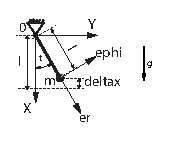
\includegraphics[height=6cm]{figures/pendulum.eps}%\hfill}\vfill}
    %\caption{With a gyroscopic solution, balance assistance is decoupled from
    %weight bearing, allowing for minimalistic hardware.}
    \caption{A pendulum consisting of a point mass and a massless rigid rod. }
    \label{fig:pendulum}%
\end{figure}


\newpart{5} \textit{What is the maximum height the point mass will reach,
measured from its bottom position, given the values} $m=\unit[2]{kg}$,
$l=\unit[9.81]{m}$, $g=\unit[9.81]{m/s^2}$?
\\

The point position can be described in polar coordinate as

\begin{equation}
    \V{r} = l\V{e}_r
\end{equation}

and it's time derivatives as

\begin{equation}
    \dot{\V{r}} = l\dot{\phi}\V{e}_{\phi}
\end{equation}
\begin{equation}
    \ddot{\V{r}} = l\ddot{\phi}\V{e}_{\phi} - l\dot{\phi}\V{e}_{r}
    \label{q1_acc}
\end{equation}

The point mass will reach its maximum height when all kinetic energy is
transferred into potential energy (As the system is only acting under the
influence of conservative forces), i.e.

\begin{equation}
    T_0 + V_0 = T_e + V_e
\end{equation}
\begin{equation}
    T_0 = \dfrac{1}{2}m\V{\dot{r}}^T\V{\dot{r}} =
        \dfrac{1}{2}ml^2\dot{\phi}^2 , T_e = 0
\end{equation}
The potential energy is defined using the resting position as reference ($\phi
= 0$)
\begin{equation}
    V_e = mg\Delta x , V_0 = 0
\end{equation}
\begin{equation}
    \Delta x =\dfrac{ l^2\dot{\phi}^2}{2g} = \unit[12.1026]{m}
\end{equation}
\begin{equation}
    x = l - \Delta x =  \unit[-2.2926]{m}
\end{equation}

\newpart{5} \textit{Derive the equations of motion for this system and solve
for angular acceleration $\ddot{\phi}$ of the rod as a function of $\phi$,
$\dot\phi$, $m$, $g,$, and $l$ using a method of your choice.}
\\\\
Using eq.\ref{q1_acc}, we can write down the equation of motion using Newton's
second law, i.e.

\begin{equation}
    m\ddot{\V{r}} = mg\left( \cos{\phi}\V{e}_r-\sin{\phi}\V{e}_{\phi} \right)
\end{equation}
\begin{equation}
    m\left( l\ddot{\phi}\V{e}_{\phi} - l\dot{\phi}\V{e}_{r}\right) =
        mg\left( \cos{\phi}\V{e}_r-\sin{\phi}\V{e}_{\phi} \right)
\end{equation}

Using the $\V{e}_{\phi}$ component

\begin{equation}
    ml\ddot{\phi} = -mg\sin{\phi}
\end{equation}
\begin{equation}
    \ddot{\phi} = -\dfrac{g}{l}\sin{\phi}
    \label{1b.ddphi}
\end{equation}

\newpart{5} \textit{Make a small-angle assumption and solve for $\phi(t)$
    analytically. Given the values $m=\unit[2]{kg}$, $l=\unit[9.81]{m}$,
    $g=\unit[9.81]{m/s^2}$, find $\phi(t_e)$ for $t_e=\unit[0.2]{s}$, with the
    above initial conditions.
}
\\
Using small angle (i.e. $\sin(\phi) = \phi$ eq. \ref{1b.ddphi} can be written
as

\begin{align}
    \ddot{\phi} &= -\dfrac{g}{l}\phi
    \\
    \ddot{\phi} +\dfrac{g}{l}\phi &= 0
    \\
    \ddot{\phi} +\omega^2\phi &=
        0 \; , \; \omega = \sqrt{\dfrac{g}{l}} = \unit[1]{rad}
\end{align}

The general solution for this 2nd order differential equation is

\begin{equation}
    \phi(t) = C\cos(\omega t+\theta)
\end{equation}

where

\begin{equation}
    \theta = \arccos\left(\phi(t_0)\right) \; , \;
    C = -\dfrac{\dot{\phi(t_0)}}{\omega\sin(\theta)}
\end{equation}

\begin{equation}
    \theta = \dfrac{\pi}{2} , \; C = -\dfrac{\pi}{2}
\end{equation}

\begin{equation}
    \phi(t) = \dfrac{\pi}{2}\sin(t)
\end{equation}

For $t_e = \unit[0.2]{s}$

\begin{equation}
    \phi(t_e) = \unit[0.3121]{rad}
\end{equation}

\newpart{3} \textit{Using the state vector $\V{x}=\begin{pmatrix} \phi
    &\dot{\phi}\end{pmatrix}^T$, re-write your (original, nonlinear) equations
        of motion in the form of a system of first-order ordinary differential
        equations (ODE).
}
\\
Eq \ref{1b.ddphi} can be written as a system of first-order ordinary
differential equations (ODE) as
\begin{align}
    \dot{y} &= v
    \\
    \dot{v} &= -\dfrac{g}{l}\sin{y}
    \label{ODEs}
\end{align}

where $y = \phi$ and $v=\dot{\phi}$
\\

\newpart{15}\textit{ Numerically integrate this ODE system by hand with the
same initial conditions, using a single step of Euler's method with step size
$h=t_e-t_0=\unit[0.2]{s}$. Compare your result for $\phi(t_e)$ to the solution
you found in the previous part of this problem. Which of the two results do you
trust more? }
\\
Using Euler's method eq. \ref{ODEs} can be written as

\begin{align}
    \dot{v}_n &= -\dfrac{g}{l}\sin(y_n)
    \\
    y_{n+1} &= y_{n} + hv_n
    \\
    v_{n+1} &= v_{n}+ h \dot{v}_n
\end{align}

As a single step is required, $y_n = \phi(t_0)$ and $v_n = \dot{\phi}(t_0)$

\begin{align}
    \dot{v}_n &= -\dfrac{g}{l}\sin(0) = 0
    \\
    y_{n+1} = y_{n} + hv_n    &= 0 + 0.2(\pi/2) = 0.1 \pi = \unit[0.3142]{rad}
    \\
    v_{n+1} = v_{n}+ h \dot{v}_n &= \pi/2 + 0.2(0) = \unit[\pi/2]{rad/s}
\end{align}

Even though both methods perform a linearisation around the equilibrium point
(i.e $\phi=0$), the linearisation using the small angle approximation still
includes the restoring effect due to gravity, while the Euler's integration
method calculates the prediction based on either the initial condition in
velocity (as this case) or the prediction in velocity (for subsequent steps).
In addition, the small angle linearisation provided an analytical solution,
while the numerical integration method is highly dependent on the step size
$h$.
\\

\newpart{2} \textit{Name two measures that could be taken (individually or in
combination) to obtain a more accurate result by numerical integration.}

\begin{itemize}
    \item Time step reduction: Reducing the time step, the truncation error is
        diminished and higher accuracy can be achieved
    \item Use more accurate integration methods: Even though reducing the time
        step leads to better accuracy, true convergence to the solution is not
        guarantee (especially for high order ODE). Thus, using more elaborated
        numerical integration algorithms (Modified Euler, Runge-Kutta,etc.)
        high accuracy and convergence can be achieved with low computational
        power (time step is not necessarily small).
\end{itemize}


\end{problem}





% ooooooooooooooooooooooooooooooooooooooooooooooooooooooooooooooo
%                           NEW PAGE
% ooooooooooooooooooooooooooooooooooooooooooooooooooooooooooooooo


%\begin{problem} {10}
%PARTICLE ON BLOCK
%\vspace{1pc}

%Do problem 1.1 from Greenwood, using the principle of virtual work and
%conservation of energy.

   % [Use conservation of linear momentum and energy.]
%\end{problem}

\newpage
\begin{problem}{30}
NUMERICAL INTEGRATION
\vspace{1pc}

First, read and understand the below example of the file {\tt
Integrate\_ModifiedEuler.m} containing the modified Euler method.

Now, implement also Euler's method and a 4th-order Runge-Kutta, in new
functions with names {\tt Integrate\_Euler.m} and {\tt
Integrate\_RungeKutta4.m}.

Integrate the sample ODE system of the ``van der Pol'' oscillator (with
$\mu=1$) for 15 seconds, with a step size of \unit[0.01]{s} and initial
conditions $\V{y}_0=\begin{pmatrix}2& 0\end{pmatrix}^T$, using this command:
\begin{lstlisting}
[t,y]=Integrate_Euler(@vanderpoldemo,[0 15],0.01,[2 0],1);%par=mu=1.
\end{lstlisting}

Report the final value of the state vector $\V{y}$ for the three different
solvers.

Using the given function {\tt Integrate\_ModifiedEuler.m} to integrate the
``van der Pol'' oscillator, gives the final result

\begin{align}
    \V{y} &= \begin{pmatrix}0.8300 & -1.3138\end{pmatrix}^T
\end{align}

The function {\tt Integrate\_Euler.m}, should look like this

\lstinputlisting{../MatlabFilesforStudents/Integrate_Euler.m}

Here lines 40 to 44 of the file {\tt Integrate\_ModifiedEuler.m} were modified
to include the euler's integration method.

\begin{align}
    \dot{y}_n &= f(y_n,t_n)
    \\
    y_{n+1} &= y_{n} + h\dot{y}_n
\end{align}

The final result using the ``van der Pol'' oscillator is

\begin{align}
    \V{y} &= \begin{pmatrix}0.9600 & -1.1969\end{pmatrix}^T
\end{align}

Analogously, the function {\tt Integrate\_RungeKutta4.m}, should look like this


\lstinputlisting{../MatlabFilesforStudents/Integrate_RungeKutta4.m}

Here lines 40 to 62 of the file {\tt Integrate\_ModifiedEuler.m} were modified
to include the 4th order Runge-Kutta's integration method.

\begin{align}
    \dot{y}_n &= f(y_n,t_n) \\
    \tilde{y}_{n+\frac{1}{2}}&=y_n+\dfrac{1}{2}h\dot{y}_n; \\
    \tilde{\dot{y}}_{n+\frac{1}{2}} &=
        f(\tilde{y}_{n+\frac{1}{2}},t_{n+\frac{1}{2}}) \\
    \tilde{\tilde{y}}_{n+\frac{1}{2}} &=
        y_n+\dfrac{1}{2} h \tilde{\dot{y}}_{n+\frac{1}{2}}; \\
    \tilde{\tilde{\dot{y}}}_{n+\frac{1}{2}} &=
        f(\tilde{\tilde{y}}_{n+\frac{1}{2}} ,t_{n+\frac{1}{2}}) \\
    \tilde{y}_{n+1}&=y_n+ h \tilde{\tilde{\dot{y}}}_{n+\frac{1}{2}}; \\
    \tilde{\dot{y}}_{n+1}&= f(\tilde{y}_{n+1},t_{n+1}) \\
    y_{n+1} &= y_{n} + \dfrac{1}{6} h \left(\dot{y}_n +
        2\tilde{\dot{y}}_{n+\frac{1}{2}} +
        2 \tilde{\tilde{\dot{y}}}_{n+\frac{1}{2}} +
        \tilde{\dot{y}}_{n+1} \right)
\end{align}

The final result using the ``van der Pol'' oscillator is

\begin{align}
    \V{y} &= \begin{pmatrix}0.8304 & -1.3134\end{pmatrix}^T
\end{align}


\end{problem}
%For a scalar initial condition $y0$ given by your student number divided by
%$10^6$.


%%%%%%%%%%%%%%%%%%%%%%%%%%%%%%%%%%%%%%%%%%%%%%%%%%%%%%%%%%%%%%%%%%%%%%%%%%%%%

\newpage


\begin{problem}{35}
{MODEL PLANE}
\vspace{1pc}

A model plane of mass $m=\unit[1]{kg}$ is suspended from the ceiling of a room
(Fig.~\ref{fig:modelplane}) by a spring with linear characteristics. The spring
has a resting length of $l_0=\unit[1]{m}$ and a spring constant
$k=\unit[20]{N/m}$. The attachment point $A$ at the ceiling is the origin of
the space-fixed $\mathcal{N}$ ($XYZ$) coordinate system. The coordinates of the
attachment point $P$ on the plane are given as (\unit[.1]{m}, 0, \unit[-.1]{m})
in the local $\mathcal{B}$ ($xyz$) coordinate system that is fixed to the
plane. The origin of the plane's local frame $\mathcal{B}$ is at the plane's
center of mass location $S$. Type I Euler angles $\psi, \theta, \phi$
(convention following Greenwood) describe the plane's orientation with respect
to the $\mathcal{N}$-frame. Gravity $g=\unit[9.81]{m/s^2}$ points in positive
$Z$-direction.


\begin{figure}[htb!]
\psfrag{x}{$x$}
\psfrag{y}{$y$}
\psfrag{z}{$z$}
\psfrag{X}{$X$}
\psfrag{Y}{$Y$}
\psfrag{Z}{$Z$}
\psfrag{P}{$P$}
\psfrag{A}{$A$}
\psfrag{g}{$g$}

\centering
    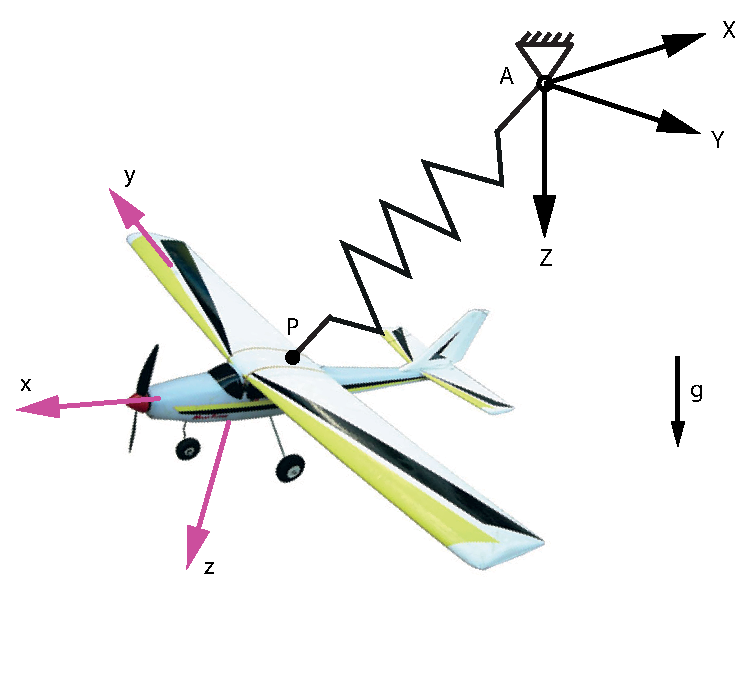
\includegraphics[height=8cm]{figures/modelplane.eps}%\hfill}\vfill}
    %\caption{With a gyroscopic solution, balance assistance is decoupled from
    %weight bearing, allowing for minimalistic hardware.}
    \caption{A model plane suspended from the ceiling. }
    \label{fig:modelplane}%
\end{figure}



Assume the plane's mass distribution is symmetric to the body-fixed $xy$ and
$xz$ planes, and the mass moments of inertia about the body-fixed axes are
$I_{xx}=I_{yy}=\frac{1}{2} I_p$, $I_{zz}=I_p$, with $I_p=\unit[.01]{kgm^2}$.
%Also, the plane is motorized and remote-controlled such that its pitch angle
%$\theta$ remains identical to zero at all times and $s_Z$ remains constant (so
%the plane is always flying parallel to the ceiling). No further control is
%applied beyond enforcing these constraints.
%
%Consider a vector $\V{q}=\begin{pmatrix}q_1 & q_2& q_3&q_4\end{pmatrix}^T$ of
%generalized coordinates that contains the Cartesian coordinates $q_1=s_X$ and
%$q_2=s_Y$ of the plane's center of mass, expressed in the space-fixed
%$\mathcal{N}$ frame, and the Euler angles $q_3=\psi$ and $q_4=\phi$ describing
%the plane's orientation with respect to the $\mathcal{N}$-frame. Use the
%Lagrange equations to find the equations of motion in the form
%$\ddot{\V{q}}=\V{f}(\V{q},\dot{\V{q}})$.
Use the Newton-Euler equations to find the linear accelerations of the plane's
center of mass, expressed in the spaced-fixed frame, as well as angular
acceleration, expressed in the body-fixed frame, as functions of the states and
external forces acting on the plane.

Then, complete the code of the function {\tt plane\_equationsofmotion.m}
(stated below), which calculates state derivatives. The function is called by
the script {\tt simulate\_plane.m} (see below).

Apply the solvers you implemented in the previous question to integrate the
equations of motion for the given initial conditions, step size, and duration
(as specified in the provided code).

By adding some lines of code at the end of {\tt simulate\_plane.m}, determine
the distance between the final center of mass positions, as obtained with
Euler's method and 4th-order Runge-Kutta. Also, calculate the principal angle
of rotation between the two calculated final orientations (so between the final
orientation obtained with Euler's method and the one obtained with
Runge-Kutta).

\vspace{.5cm}
\textbf{The code that must be included is highlighted with blue.}
\begin{lstlisting}[escapechar=!]
function dx=plane_equationsofmotion(t,x,par)
%function dx=plane_equationsofmotion(t,x,par)
%This function contains the equations of motion of a model airplane
%connected to the ceiling by a linear spring, as used in homework
%assignments of the course "Advanced Dynamics" at TUD.
%
%Input: t (time) and
%x: Cartesian positions, Euler angles, linear speeds, omega
%Output: dx: derivatives thereof
%
%H. Vallery, October 2014
%Modified by Daniel Lemus, Oct 2014

%----------------------------
%extract parameters:
%----------------------------

g=par.g;%[m/s^2], acceleration of gravity (points in positive z direction)

%spring parameters:
l0=par.l0;%m, resting length of spring
k=par.k;%N/m, stiffness of spring
rp_B=par.rp_B;%position vector of point P (spring attachment point) in B frame

%mass parameters of the plane:
m=par.m;% mass of plane
Ixx=par.Ixx;% moment of inertia about x axis
Iyy=par.Iyy;% moment of inertia about y axis
Izz=par.Izz;% moment of inertia about z axis

%----------------------------
%read current states:
%----------------------------

sX=x(1);
sY=x(2);
sZ=x(3);
psi=x(4);
theta=x(5);
phi=x(6);

dsX=x(7);
dsY=x(8);
dsZ=x(9);
omegax=x(10);
omegay=x(11);
omegaz=x(12);

rs_N=[sX;sY;sZ];%position of point S (center of mass) in N coordinates

%----------------------------
%calculate forces and moments in body frame:
%----------------------------

%construction of rotation matrix that maps vectors that are
%expressed in the N frame to their representation in the B frame:

R_psi= !\colorbox{light-red}{[cos(psi) sin(psi) 0;-sin(psi) cos(psi) 0; 0 0 1];}!
R_theta= !\colorbox{light-red}{[cos(theta) 0 -sin(theta);0 1 0;sin(theta) 0 cos(theta)];}!
R_phi= !\colorbox{light-red}{[1 0 0; 0 cos(phi) sin(phi); 0 -sin(phi) cos(phi)];}!
R_total= !\colorbox{light-red}{R\_phi*R\_theta*R\_psi;}!

%position vector of point P in the N frame:
rp_N=!\colorbox{light-red}{rs\_N+R\_total'*rp\_B;}!

%external forces acting on the plane:
e_spring = !\colorbox{light-red}{-rp\_N/norm(rp\_N);}!
dl = !\colorbox{light-red}{norm(rp\_N)- l0;}!
Fspring_N= !\colorbox{light-red}{k * dl * e\_spring;}!%spring force in the N frame
Fg_N=[0;0;m*g];%gravitational force in the N frame
Ftot_N=(Fspring_N+Fg_N);%total force in the N frame

%map the spring force to the body frame:
Fspring_B= !\colorbox{light-red}{R\_total*Fspring\_N;}!%spring force in the body frame

%calculate the external moments acting about the plane's center of mass:
M=cross(!\colorbox{light-red}{rp\_B,Fspring\_B}!);%moment of the spring in the body frame
%components about the body-fixed axes:
Mx=M(1);My=M(2);Mz=M(3);

%----------------------------
%apply Newton-Euler:
%----------------------------

%Newton equations (in space-fixed frame):
ddsX=!\colorbox{light-red}{Ftot\_N(1)/m;}!
ddsY=!\colorbox{light-red}{Ftot\_N(2)/m;}!
ddsZ=!\colorbox{light-red}{Ftot\_N(3)/m;}!

%Euler equations (in body-fixed frame):
domegax= !\colorbox{light-red}{(Mx-(Izz-Iyy)*omegay*omegaz)/Ixx;}!
domegay= !\colorbox{light-red}{(My-(Ixx-Izz)*omegax*omegaz)/Iyy;}!
domegaz= !\colorbox{light-red}{(Mz-(Iyy-Ixx)*omegax*omegay)/Izz;}!

%----------------------------
%calculate state derivatives:
%----------------------------

%Euler angle derivatives, Greenwood (3.16)
dpsi=sec(theta)* (omegay*sin(phi)+omegaz*cos(phi));
dtheta = omegay*cos(phi)-omegaz*sin(phi);
dphi = omegax + dpsi *sin(theta);

dx=[dsX;dsY;dsZ;dpsi;dtheta;dphi;ddsX;ddsY;ddsZ;domegax;domegay;domegaz];


\end{lstlisting}


The function is called by this script {\tt simulate\_plane.m}:

\begin{lstlisting}[escapechar=!]


%This script simulates a model plane connected to the ceiling by a linear
%spring, as treated in homework assignments of the course "Advanced
%Dynamics" at TUD.
%Author: H. Vallery, October 2014
%Modified: D. Lemus, Oct 2014

%----------------------------
%define constant parameters:
%----------------------------
Ts=.01;%[s], sampling time
endtime=0.5;%[s] %end time of integration
par.Ts_anim=.01;%[s] pause between frames during animation (can be used for slow motion if larger than Ts)

%gravity:
par.g=9.81;%[m/s^2] acceleration of gravity (points in positive z direction)

%mass properties:
Ip=1*.1^2;%[kgm^2] moment of inertia of the plane about the z axis
par.Ixx=.5*Ip;
par.Iyy=.5*Ip;
par.Izz=Ip;

par.m=1;%[kg], mass of the plane

%geometry:
px=.1;%[m] local x coordinate of point P (spring attachment point) in B frame
pz=-.1;%[m] local z coordinate of P
par.rp_B=[px;0;pz];%coordinates of point P in B frame

par.l0=1;%[m], resting length of spring
par.k=20;%[N/m], stiffness of spring

%additional geometric data for aninmation of the plane:
par.length_plane=2;%[m], length of the plane's body
par.wingspan=4;%[m] wingspan
par.height_fin=.5;%[m] height of the fin
par.r_wingcenter=[.1;0;-.01];%[m] vector from CoM to wing center in body frame


%----------------------------
%set initial conditions:
%----------------------------

%Cartesian positions of the plane's center of mass:
sX=-px;
sY=.2;%.2;
sZ=par.l0+par.m*par.g/par.k;
%corresponding velocities:
dsX=2;
dsY=0;
dsZ=0;
%Euler angles (type I) to describe the orientation of the plane with
%respect to the inertial N frame (XYZ):
psi=0*pi/3;%rotation about Z axis
theta=0*pi/20;%rotation about intermediate Y' axis
phi=0*pi/10;%rotation about new x axis
%angular velocities (expressed in the body-fixed B frame (xyz) of the plane):
omegax=0;
omegay=0;
omegaz=pi/4/10;

%----------------------------
%integrate:
%----------------------------
x0=[sX,sY,sZ,psi,theta,phi,dsX,dsY,dsZ,omegax,omegay,omegaz];%vector of initial conditions:
options = odeset('AbsTol',1e-10,'RelTol',1e-8);
%[t,y]=ode45(@plane_equationsofmotion,[0:Ts:endtime],x0,options,par);
!\colorbox{light-red}{[t,y0] = Integrate\_Euler(@plane\_equationsofmotion,[0,endtime],Ts, x0,par);}!
%[t,y] = Integrate_ModifiedEuler(@plane_equationsofmotion,[0,endtime],Ts, x0,par);
%[t,y] = Integrate_RungeKutta2(@plane_equationsofmotion,[0,endtime],Ts, x0,par);
!\colorbox{light-red}{[t,y1] = Integrate\_RungeKutta4(@plane\_equationsofmotion,[0,endtime],Ts, x0,par);}!

%extract the generalized coordinates as time series:
qmatrix0=y0(:,1:6);
qmatrix1=y1(:,1:6);

%----------------------------
%animate the result:
%----------------------------
planeanimation(qmatrix0,par);
planeanimation(qmatrix1,par);

% Define Rotation Matrix for Euler angles type I
!\colorbox{light-red}{R\_psi = @(psi) [cos(psi) sin(psi) 0;-sin(psi) cos(psi) 0; 0 0 1];}!
!\colorbox{light-red}{R\_theta= @(theta) [cos(theta) 0 -sin(theta);0 1 0;sin(theta) 0 cos(theta)];}!
!\colorbox{light-red}{R\_phi= @(phi) [1 0 0; 0 cos(phi) sin(phi); 0 -sin(phi) cos(phi)];}!


!\colorbox{light-red}{x0 = y0(end,1:3);}!
!\colorbox{light-red}{psi = y0(end,4);}!
!\colorbox{light-red}{theta = y0(end,5);}!
!\colorbox{light-red}{phi = y0(end,6);}!

% Rotation Matrix final orientation euler's integration method
!\colorbox{light-red}{R\_N2E= R\_phi(phi)*R\_theta(theta)*R\_psi(psi);}!

!\colorbox{light-red}{x1 = y1(end,1:3);}!
!\colorbox{light-red}{psi = y1(end,4);}!
!\colorbox{light-red}{theta = y1(end,5);}!
!\colorbox{light-red}{phi = y1(end,6);}!

% Rotation Matrix final orientation RK4 integration method
!\colorbox{light-red}{R\_N2RK= R\_phi(phi)*R\_theta(theta)*R\_psi(psi);}!

% Rotation Matrix from Euler to RK4 final orientations
!\colorbox{light-red}{R = R\_N2RK*R\_N2E';}!

% principal angle of rotation
!\colorbox{light-red}{phi = acos((trace(R)-1)*0.5);}!

% Distance between final center of mass postions Euler and RK4 integration
% methods
!\colorbox{light-red}{dist = norm(x1-x0);}!

disp(sprintf('instantaneous angle of rotation = %g',phi))
disp(sprintf('final disance = %g',dist))

\end{lstlisting}

The animation function {\tt planeanimation.p} is also provided (closed source).

The output of {\tt simulate\_plane.m} is:
\begin{align*}
    \phi &= \unit[2.95089]{rad} \\
    \text{final distance} &= \unit[0.132272]{m}
\end{align*}


\end{problem}

\newpage

\begin{problem}{50}
BONUS PROBLEM: THREEWHEELER
\vspace{1pc}

We consider a three-wheeled cart with massless wheels, as treated in the
lecture of week 7 (Fig.\ref{fig:threewheeler}), which moves in the horizontal
($XY$) plane. The front wheel at point $C$ is an actuated omni-wheel, while the
unactuated rear wheels at the corners $A$ and $B$ roll in direction of the
body-fixed $x$-axis, without slip in any of the horizontal directions. The
cart's instantaneous configuration is described by a vector of generalized
coordinates $\V{q}=\begin{pmatrix}s_X & s_Y & \theta \end{pmatrix}^T$. The
components $s_X$ and $s_Y$ describe the position of the cart's center of mass
$S$, expressed in the space-fixed $\mathcal{N}$-frame, and $\theta$ is the
heading angle. The omni-wheel is actuated in such a way that the ground exerts
friction forces $F_x$ and $F_y$ on the the cart at point $C$. Assume the cart
has a mass $m$, and it is a block of homogeneous material, with length $l$ and
width $d$. You may re-use and refer to the constraint equation as derived in
the lecture.

\begin{figure}[htb!]
\psfrag{x}{$x$}
\psfrag{y}{$y$}
\psfrag{v}{$s_X$}
\psfrag{w}{$s_Y$}
\psfrag{0}{$0$}
\psfrag{d}{$\frac{d}{2}$}
\psfrag{l}{$\frac{l}{2}$}
\psfrag{X}{$X$}
\psfrag{Y}{$Y$}
\psfrag{m}{$m$}
\psfrag{S}{$S$}
\psfrag{F}{$F_x$}
\psfrag{G}{$F_y$}
\psfrag{A}{$A$}
\psfrag{B}{$B$}
\psfrag{C}{$C$}
\psfrag{t}{$\theta$}

\centering
    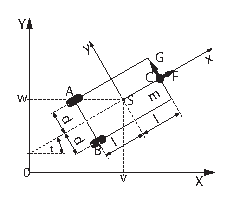
\includegraphics[height=8cm]{figures/threewheeler.eps}%\hfill}\vfill}
    %\caption{With a gyroscopic solution, balance assistance is decoupled from
    %weight bearing, allowing for minimalistic hardware.}
    \caption{A three-wheeled cart moving in the horizontal plane. }
    \label{fig:threewheeler}%
\end{figure}

The function {\tt cart\_equationsofmotion.m} that calculates state derivatives,
the animation function {\tt cartanimation.m}, and the script {\tt
simulate\_cart.m} that calls the two functions are provided. The files
currently generate movement of the cart for a constant force at the omni-wheel
in negative $y$-direction, as used to generate one of the videos shown in the
lecture. Within this exercise, you will modify the code to investigate a
different movement.

\newpart{5}
Assume the cart now moves backwards in such a way that $s_X=-v_0 t$ and
$\theta=\pi/8\sin(2\pi f t)$, with the constant parameters $v_0=\unit[20]{m/s}$
and $f=\unit[2]{Hz}$. The initial $Y$-position $s_Y(t_0)$ of the center of mass
$S$ at $t_0=0$ is 0. Find the initial velocity $\dot{s}_Y(t_0)$ of the cart at
$t_0=0$ such that the constraint equation (as derived in the lecture) is
fulfilled. You should do this by replacing the code in the definition of
initial conditions in {\tt simulate\_cart.m}.

\newpart{15}
Write a new function {\tt inversedynamics\_cart.m} that is called by {\tt
simulate\_cart.m} and use it to calculate the applied forces $F_x$ and $F_y$ in
the body-fixed frame that are needed to generate the above movement, for
$N=500$ samples of time (with a sampling rate of $Ts=\unit[0.01]{s}$). What are
the final values for $F_x$ and $F_y$ (so at $t_e=(N-1)\cdot Ts$)?

\vspace{.3cm}
\emph{Hint:} Your function should have a header like this, and it should return
scalar values for forces when provided scalar values of kinematic data:
\begin{lstlisting}
function [Fx,Fy]=inversedynamics_cart(theta,ddsX,ddsY,domega,par)
%This function calculates forces Fx and Fy as functions of given motion
%(not checking for violation of constraints!)
%par: parameter struct containing length and mass properties of the cart
\end{lstlisting}
Call it within a loop in {\tt simulate\_cart.m}.

\newpart{15}
Add the calculated forces as a matrix with $N$ rows and 2 columns (containing
the components $F_x$ and $F_y$) as another parameter in the Matlab structure
{\tt par}.

Then, with the same initial conditions (also including the velocity component
$\dot{s}_Y(t_0)$ you found in the first part of this problem), apply these
forces again in the forward simulation (by reading out the matrix entries from
{\tt par} in the equations of motion), using the Modified Euler Method for the
$N$ samples of time. Finally, calculate the absolute error between the final
center of mass $X$-component $\hat{s}_{X}(t_e)$ of the cart, as calculated in
the forward simulation, and the true value $s_X(t_e)=-v_0 t_e$, with
$t_e=(N-1)\cdot Ts$.

\newpart{15}
Calculate the constraint force acting on the rear axle of the cart for the $N$
samples of your forward simulation. What is the maximum absolute value of this
constraint force?

Assuming a constant vertical contact force at each contact point due to weight
of the cart (so neglecting the dynamic shifting of weight between the three
wheels), and assuming a friction coefficient of $\mu=0.7$ and acceleration of
gravity $g=\unit[9.81]{m/s^2}$ pointing in negative $Z$ direction, do you think
the assumption of no slip at the rear wheels was valid?

\vspace{.5cm}

Content of the file {\tt simulate\_cart.m}:
\begin{lstlisting}
%This script simulates a three-wheeled cart,
%as treated in week 7 of the course "Advanced
%Dynamics" at TUD.
%Author: H. Vallery, October 2014


%----------------------------
%define constant parameters:
%----------------------------
Ts=.04;%[s], sampling time
endtime=10;%[s] %end time of integration
par.Ts_anim=.04;%[s] pause between frames during animation
%(can be used for slow motion if larger than Ts)


%geometry:

par.length_cart=2;%[m], length of the cart
par.width_cart=1;%[m] width of the cart

%mass properties:
par.m=20;%[kg], mass of the cart
par.Is=par.m*1/12*(par.length_cart^2+par.width_cart^2);%[kgm^2] moment of inertia
%of the cart about the z axis

%----------------------------
%set initial conditions:
%----------------------------

%Cartesian positions of the cart's center of mass:
sX=0;%[m]
sY=.2;%[m]
%corresponding velocities:
dsX=2;%[m/s]
dsY=2;%[m/s]

%orientation of the cart with
%respect to the inertial N frame (XYZ):
theta=0;%[rad], rotation about z axis
%angular velocity:
omega=2;%[rad/s]
%Remark: These initial conditions fulfill the given constraint

%----------------------------
%integrate:
%----------------------------
x0=[sX,sY,theta,dsX,dsY,omega];%vector of initial conditions:
options = odeset('AbsTol',1e-10,'RelTol',1e-8);
%[t,y]=ode45(@cart_equationsofmotion,[0:Ts:endtime],x0,options,par);
%[t,y] = Integrate_Euler(@cart_equationsofmotion,[0,endtime],Ts, x0,par);
[t,y] = Integrate_ModifiedEuler(@cart_equationsofmotion,[0,endtime],Ts, x0,par);
%[t,y] = Integrate_RungeKutta2(@cart_equationsofmotion,[0,endtime],Ts, x0,par);
%[t,y] = Integrate_RungeKutta4(@cart_equationsofmotion,[0,endtime],Ts, x0,par);


%extract the generalized coordinates as time series:
qmatrix=y(:,1:3);

%----------------------------
%animate the result:
%----------------------------

cartanimation(qmatrix,par);
\end{lstlisting}
\end{problem}


%welke krachten en momenten nodig om sinusvormige beweging te maken, dan deze
%week

Content of the file {\tt cart\_equationsofmotion.m}:
\begin{lstlisting}
function dx=cart_equationsofmotion(t,x,par)
%function dx=cart_equationsofmotion(t,x,par)
%This function contains the 2D equations of motion of a three-wheeled cart
%driving around on the ground, as used in homework
%assignments of the course "Advanced Dynamics" at TUD.
%
%Inputs:
%t (time)
%state vector x: Cartesian x/y positions (in m) of cart center of mass,
% heading angle theta (in rad), & corresponding velocities (in m/s, rad/s).
%par: parameter struct containing length and mass properties of the cart
%
%Output: dx: derivatives of the states
%
%Author: H. Vallery, October 2014

%----------------------------
%extract parameters:
%----------------------------

%mass parameters of the cart:
m=par.m;% mass of cart
Is=par.Is;% moment of inertia about center of mass

%geometry of the cart:
l=par.length_cart;%[m], length of the cart
%d=par.width_cart;%[m] width of the cart, not needed


%----------------------------
%read current states:
%----------------------------

sX=x(1);
sY=x(2);
theta=x(3);

dsX=x(4);
dsY=x(5);
omega=x(6);

%----------------------------
%Lagrange:
%----------------------------

Fx=-50;%[N], forward force
Fy=0;%[N], steering force

%for steering movie:
%Fx=0;%forward force
%Fy=-50;%steering force

%for backward movie:
%Fx=-50;%forward force
%Fy=0;%steering force


A=[m 0 -2*Is/l*sin(theta);
    0 m 2*Is/l*cos(theta);
    sin(theta) -cos(theta) l/2];

b=[ Fx*cos(theta) - 2*Fy*sin(theta);
    Fx*sin(theta)+2*Fy*cos(theta);
    -dsX*omega*cos(theta)-dsY*omega*sin(theta)];

ddq=A\b;
ddsX=ddq(1);
ddsY=ddq(2);
domega=ddq(3);


%----------------------------
%calculate state derivatives:
%----------------------------

dx=[dsX;dsY;omega;ddsX;ddsY;domega];



\end{lstlisting}


\newpage

%\vfill

\clearpage

\showpoints
\end{document}



